\documentclass[10pt]{article} 
\usepackage{fontspec}

\usepackage{mdframed}
\usepackage{amsmath}
\usepackage[space]{xeCJK}
\setCJKmainfont{Noto Sans KR}
\usepackage[a4paper, margin=1in]{geometry}
\setlength{\parindent}{10pt}
\usepackage{graphicx}
\usepackage{setspace}
\usepackage[breakable,skins]{tcolorbox}
\usepackage{enumitem}
\usepackage{cancel}
\usepackage{xcolor}
\usepackage{float}
\usepackage{mathrsfs}
\usepackage{subcaption}
\usepackage{amssymb}
\usepackage{tabularx}   % X 열 타입 제공
\usepackage{booktabs}   % 선택사항: 예쁜 선을 위해
\usepackage[colorlinks=true, linkcolor=blue, urlcolor=cyan]{hyperref}


\setstretch{1.3}
\setlength{\jot}{6pt}
\title{
  2025 남도여행 숙소 : 순천
}

\author{
  Yoonho Choi \and
  Seoin Choi 
}

\date{
  Mathematical Science Lab, Department of appiled physics\\
  Hanyang University, Ansan, Republic of Korea\\[1ex]
  July 28, 2025
}


\begin{document}


\maketitle

\section{Abstract}
본 문서는 2025 8/1(토) \(\thicksim\) 8/3(월) 총 3일간 예정되어있는 남도여행 일정중 8/1(토) \(\thicksim\) 8/2(일) 순천에서의 숙박에 관한 정리이다. 
우선 가격대별로 저렴한 숙소들을 나열하고, 조금더 가격대가 있지만, 숙소의 퀄리티가 좋은곳들을 소개한다. 
각 숙소에 대한 설명으로는 예약 가능한 가격, 여기어때 평점, 위치등을 포함한다. 

\section{Introduction}
어제 전남투어 어플리케이션에 올라와있는 펜션을 제외한 모든 숙소를 찾아본 결과, 대략적으로는 크게 5\(\thicksim\)6만원 정도의 숙소 (쿠폰 적용시 3만원 \(\thicksim\) 3만 5천원) 선의 숙소가 있고, 
이 다음으로는 바로 8만원(쿠폰 적용시 5만원) , 10만원(쿠폰 적용시 6만원) 정도의 숙소가 있어서, 어떻게 할지 결정해야한다. 
이후의 가격은 쿠폰이 적용된 가격으로 표기한다. 
\newpage

\section{accommodation}
\subsection{3만원대 숙소}
\subsubsection{순천 테라칸}
\begin{figure}[htbp]
  \centering
  % 첫 번째 그림
  \begin{subfigure}{0.3\textwidth}
    \centering
    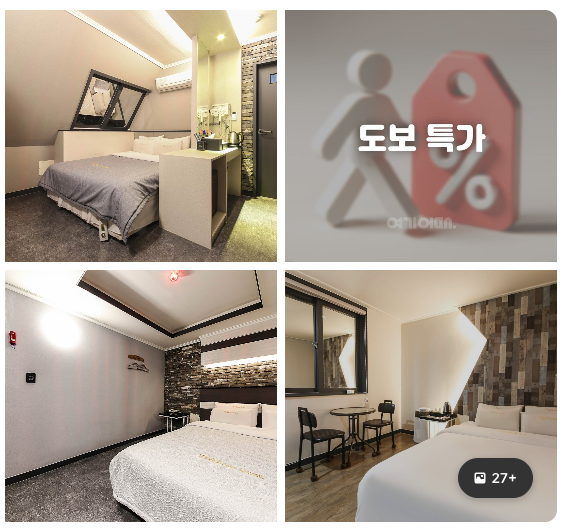
\includegraphics[width=\linewidth]{fig/순천테라칸_방.png}
    \caption{방 사진}
    \label{fig:1}
  \end{subfigure}
  \hfill
  % 두 번째 그림
  \begin{subfigure}{0.3\textwidth}
    \centering
    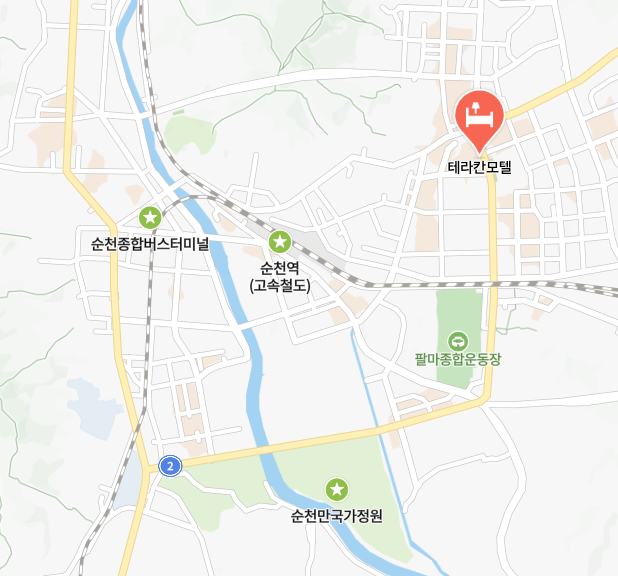
\includegraphics[width=\linewidth]{fig/순천테라칸_위치.png}
    \caption{위치}
    \label{fig:2}
  \end{subfigure}
  \hfill
  % 세 번째 그림
  \begin{subfigure}{0.3\textwidth}
    \centering
    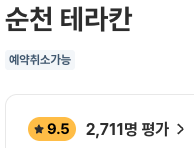
\includegraphics[width=\linewidth]{fig/순천테라칸_후기.png}
    \caption{여기어때 후기}
    \label{fig:3}
  \end{subfigure}
  \label{fig:three}
\end{figure}
\begin{center}
\textbf{할인 적용 가격 : 35000}
\end{center}
\url{https://www.yeogi.com/domestic-accommodations?keyword=%EC%88%9C%EC%B2%9C+%ED%85%8C%EB%9D%BC%EC%B9%B8&checkIn=2025-08-02&checkOut=2025-08-03&personal=2&freeForm=true}

\bigskip      % 옵션: 위·아래 여백 조절
\hrule        % 기본 두께의 수평선
\bigskip

\subsubsection{순천 S 무인호텔}
\begin{figure}[htbp]
  \centering
  % 첫 번째 그림
  \begin{subfigure}{0.3\textwidth}
    \centering
    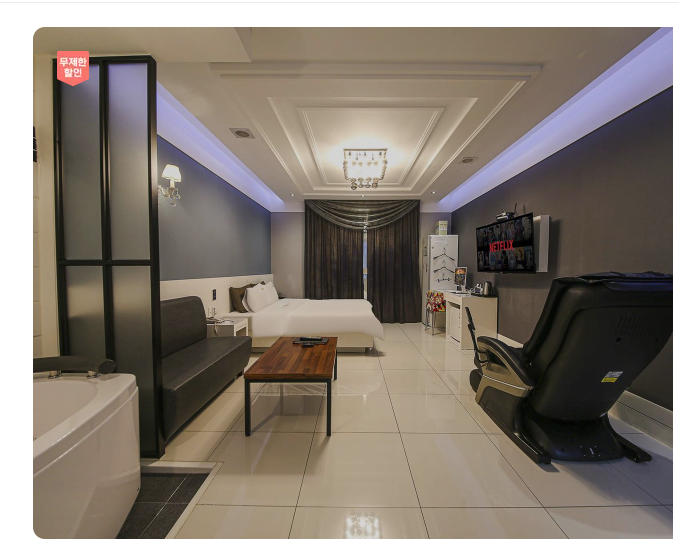
\includegraphics[width=\linewidth]{fig/순천S무인호텔_방.png}
    \caption{방 사진}
    \label{fig:1}
  \end{subfigure}
  \hfill
  % 두 번째 그림
  \begin{subfigure}{0.3\textwidth}
    \centering
    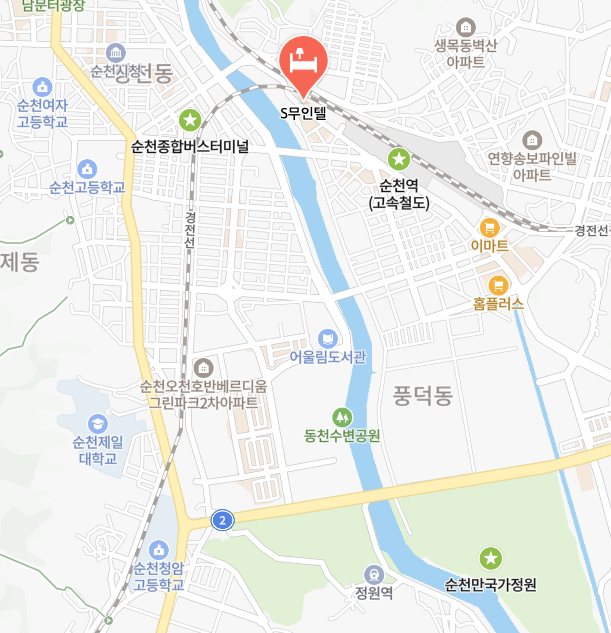
\includegraphics[width=\linewidth]{fig/순천S무인호텔_위치.png}
    \caption{위치}
    \label{fig:2}
  \end{subfigure}
  \hfill
  % 세 번째 그림
  \begin{subfigure}{0.3\textwidth}
    \centering
    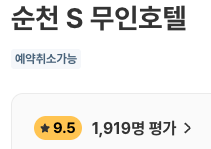
\includegraphics[width=\linewidth]{fig/순천S무인호텔_후기.png}
    \caption{여기어때 후기}
    \label{fig:3}
  \end{subfigure}
  \label{fig:three}
\end{figure}
\begin{center}
\textbf{할인 적용 가격 : 32000}
\end{center}
\url{https://www.yeogi.com/domestic-accommodations/4699?checkIn=2025-08-02&checkOut=2025-08-03&personal=2}

\newpage

\subsubsection{순천 써드 호텔}
\begin{figure}[htbp]
  \centering
  % 첫 번째 그림
  \begin{subfigure}{0.3\textwidth}
    \centering
    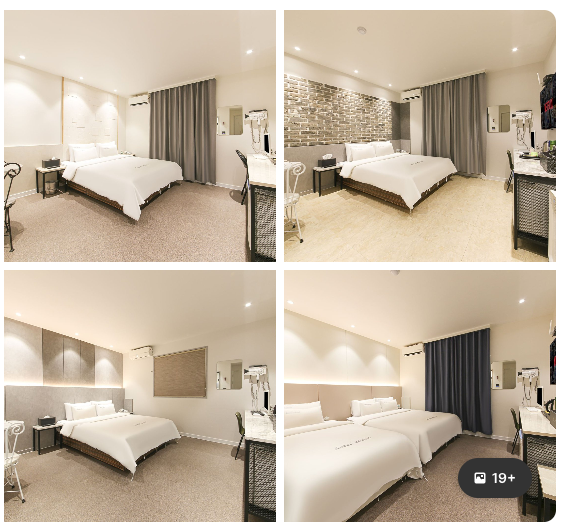
\includegraphics[width=\linewidth]{fig/6_방.png}
    \caption{방 사진}
    \label{fig:1}
  \end{subfigure}
  \hfill
  % 두 번째 그림
  \begin{subfigure}{0.3\textwidth}
    \centering
    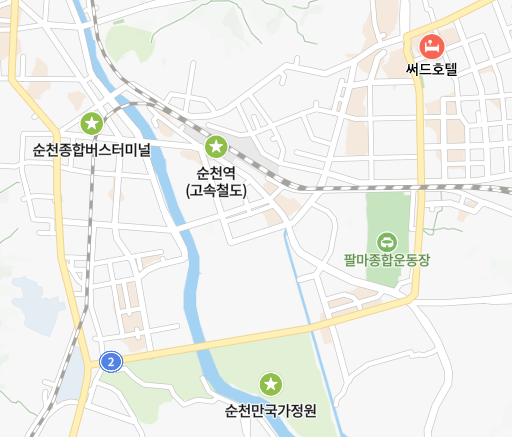
\includegraphics[width=\linewidth]{fig/6_위치.png}
    \caption{위치}
    \label{fig:2}
  \end{subfigure}
  \hfill
  % 세 번째 그림
  \begin{subfigure}{0.3\textwidth}
    \centering
    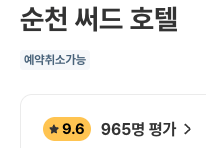
\includegraphics[width=\linewidth]{fig/6_후기.png}
    \caption{여기어때 후기}
    \label{fig:3}
  \end{subfigure}
  \label{fig:three}
\end{figure}
\begin{center}
\textbf{할인 적용 가격 : 40000}
\end{center}
\url{https://www.yeogi.com/domestic-accommodations/66668?checkIn=2025-08-02&checkOut=2025-08-03&personal=2}

\bigskip      % 옵션: 위·아래 여백 조절
\hrule        % 기본 두께의 수평선
\bigskip

\subsubsection{순천 69}
\begin{figure}[htbp]
  \centering
  % 첫 번째 그림
  \begin{subfigure}{0.3\textwidth}
    \centering
    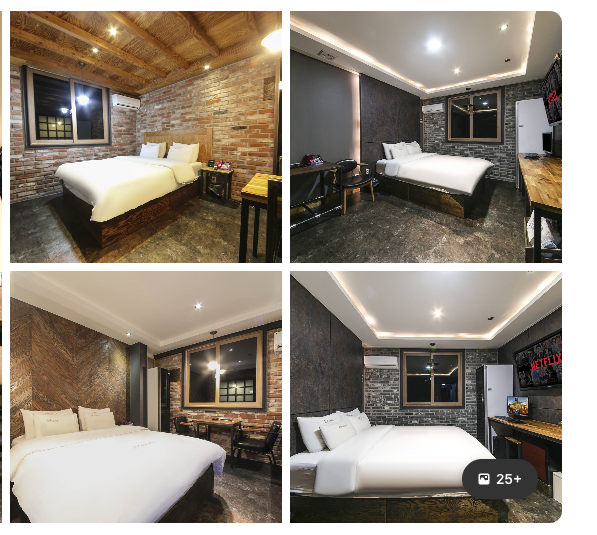
\includegraphics[width=\linewidth]{fig/7_방.png}
    \caption{방 사진}
    \label{fig:1}
  \end{subfigure}
  \hfill
  % 두 번째 그림
  \begin{subfigure}{0.3\textwidth}
    \centering
    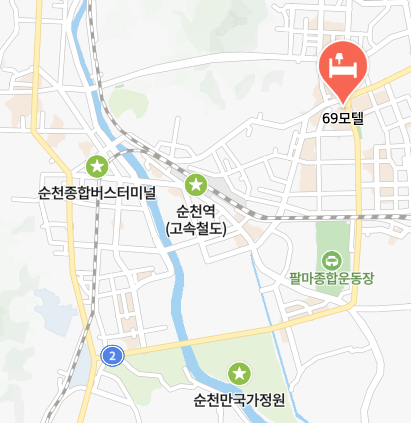
\includegraphics[width=\linewidth]{fig/7_위치.png}
    \caption{위치}
    \label{fig:2}
  \end{subfigure}
  \hfill
  % 세 번째 그림
  \begin{subfigure}{0.3\textwidth}
    \centering
    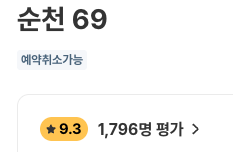
\includegraphics[width=\linewidth]{fig/7_후기.png}
    \caption{여기어때 후기}
    \label{fig:3}
  \end{subfigure}
  \label{fig:three}
\end{figure}
\begin{center}
\textbf{할인 적용 가격 : 40000}
\end{center}
\url{https://www.yeogi.com/domestic-accommodations/3680?checkIn=2025-08-02&checkOut=2025-08-03&personal=2}

\newpage

\subsection{5만원대 숙소}
\subsubsection{순천 YAJA 순천조례점}
\begin{figure}[htbp]
  \centering
  % 첫 번째 그림
  \begin{subfigure}{0.3\textwidth}
    \centering
    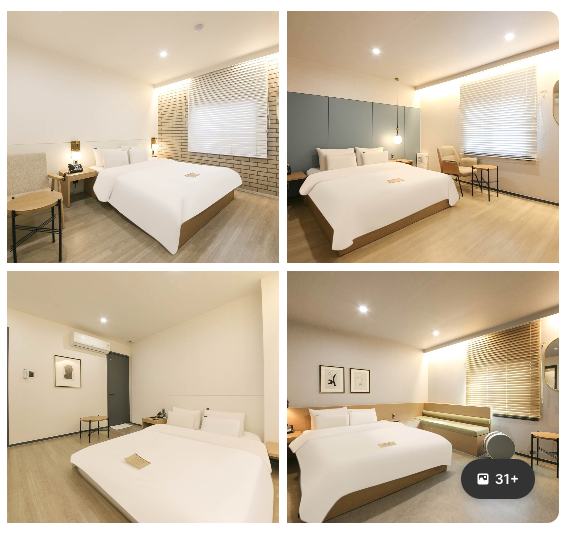
\includegraphics[width=\linewidth]{fig/8_방.png}
    \caption{방 사진}
    \label{fig:1}
  \end{subfigure}
  \hfill
  % 두 번째 그림
  \begin{subfigure}{0.3\textwidth}
    \centering
    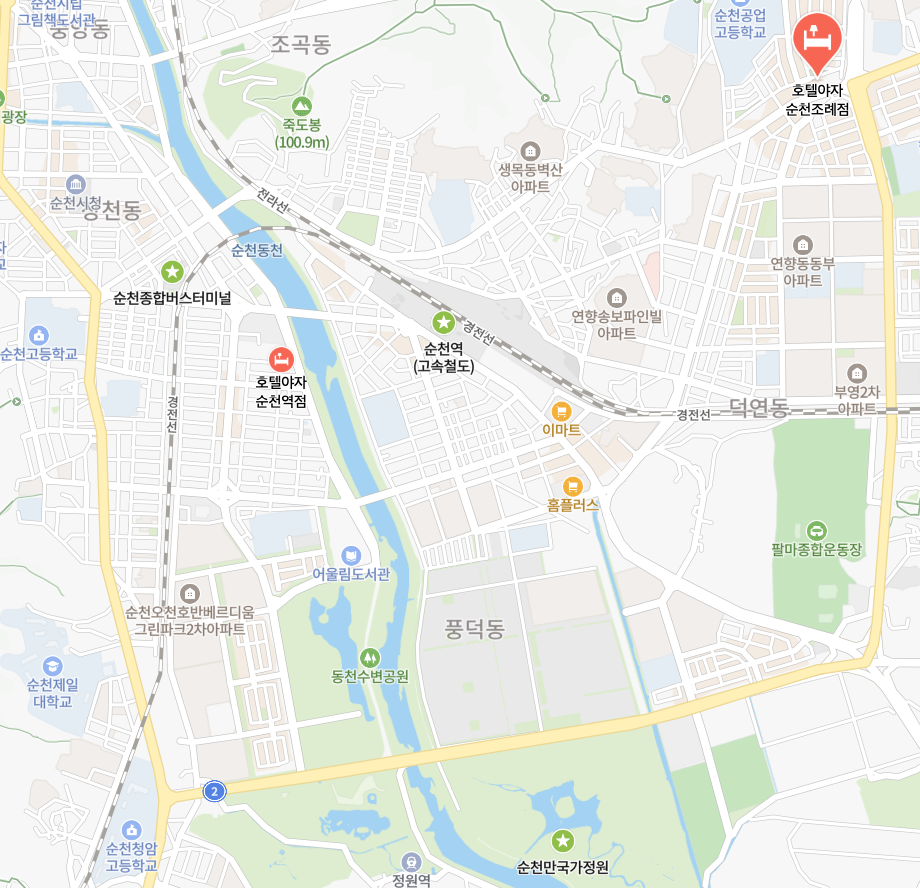
\includegraphics[width=\linewidth]{fig/8_위치.png}
    \caption{위치}
    \label{fig:2}
  \end{subfigure}
  \hfill
  % 세 번째 그림
  \begin{subfigure}{0.3\textwidth}
    \centering
    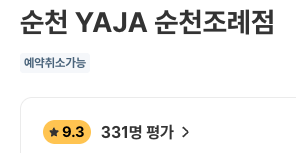
\includegraphics[width=\linewidth]{fig/8_후기.png}
    \caption{여기어때 후기}
    \label{fig:3}
  \end{subfigure}
  \label{fig:three}
\end{figure}
\begin{center}
\textbf{할인 적용 가격 : 50000}
\end{center}
\url{https://www.yeogi.com/domestic-accommodations/73816?checkIn=2025-08-02&checkOut=2025-08-03&personal=2}
\bigskip      % 옵션: 위·아래 여백 조절
\hrule        % 기본 두께의 수평선
\bigskip
\subsubsection{순천 호텔 본}
\begin{figure}[htbp]
  \centering
  % 첫 번째 그림
  \begin{subfigure}{0.3\textwidth}
    \centering
    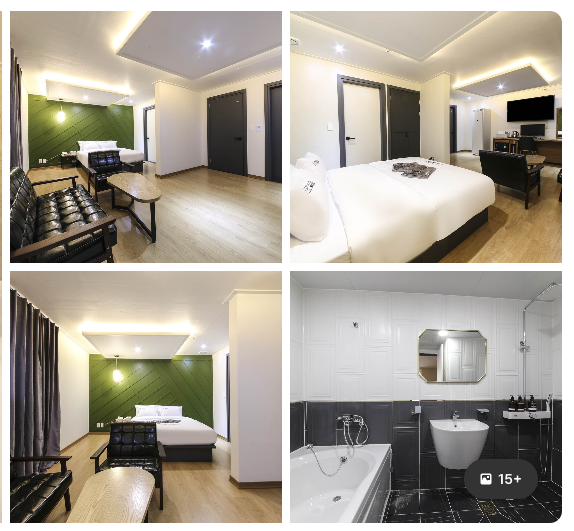
\includegraphics[width=\linewidth]{fig/3_방.png}
    \caption{방 사진}
    \label{fig:1}
  \end{subfigure}
  \hfill
  % 두 번째 그림
  \begin{subfigure}{0.3\textwidth}
    \centering
    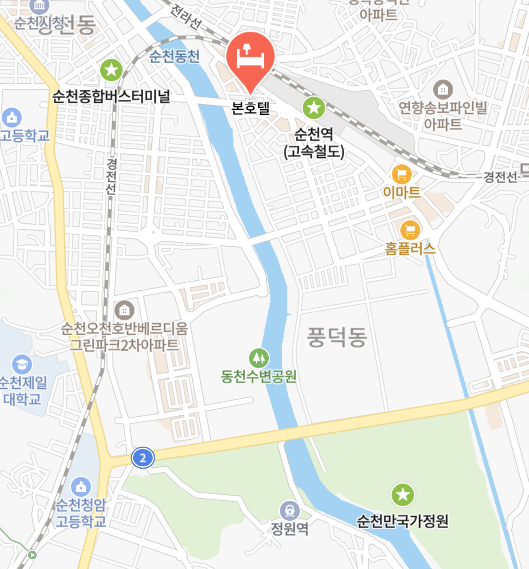
\includegraphics[width=\linewidth]{fig/3_위치.png}
    \caption{위치}
    \label{fig:2}
  \end{subfigure}
  \hfill
  % 세 번째 그림
  \begin{subfigure}{0.3\textwidth}
    \centering
    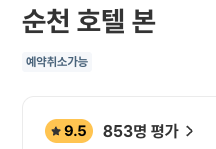
\includegraphics[width=\linewidth]{fig/3_후기.png}
    \caption{여기어때 후기}
    \label{fig:3}
  \end{subfigure}
  \label{fig:three}
\end{figure}
\begin{center}
\textbf{할인 적용 가격 : 52000}
\end{center}
\url{https://www.yeogi.com/domestic-accommodations?keyword=%EC%88%9C%EC%B2%9C+%ED%98%B8%ED%85%94+%EB%B3%B8&checkIn=2025-08-02&checkOut=2025-08-03&personal=2&freeForm=true}

\newpage
\subsection{6만원대 숙소}
\subsubsection{브라운도트호텔 정원박람회점}
\begin{figure}[htbp]
  \centering
  % 첫 번째 그림
  \begin{subfigure}{0.3\textwidth}
    \centering
    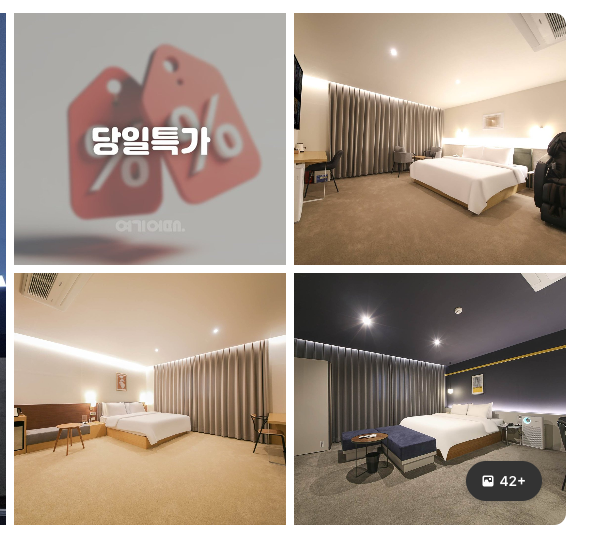
\includegraphics[width=\linewidth]{fig/4_방.png}
    \caption{방 사진}
    \label{fig:1}
  \end{subfigure}
  \hfill
  % 두 번째 그림
  \begin{subfigure}{0.3\textwidth}
    \centering
    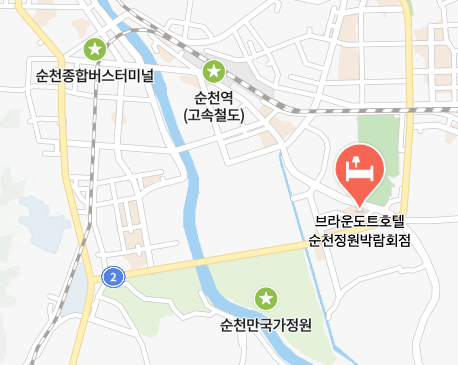
\includegraphics[width=\linewidth]{fig/4_위치.png}
    \caption{위치}
    \label{fig:2}
  \end{subfigure}
  \hfill
  % 세 번째 그림
  \begin{subfigure}{0.3\textwidth}
    \centering
    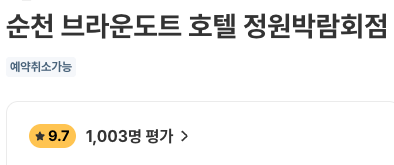
\includegraphics[width=\linewidth]{fig/4_후기.png}
    \caption{여기어때 후기}
    \label{fig:3}
  \end{subfigure}
  \label{fig:three}
\end{figure}
\begin{center}
\textbf{할인 적용 가격 : 60000}
\end{center}
\url{https://www.yeogi.com/domestic-accommodations/69243?checkIn=2025-08-02&checkOut=2025-08-03&personal=2}
\bigskip      % 옵션: 위·아래 여백 조절
\hrule        % 기본 두께의 수평선
\bigskip

\subsubsection{순천 호텔 Moon}
\begin{figure}[htbp]
  \centering
  % 첫 번째 그림
  \begin{subfigure}{0.3\textwidth}
    \centering
    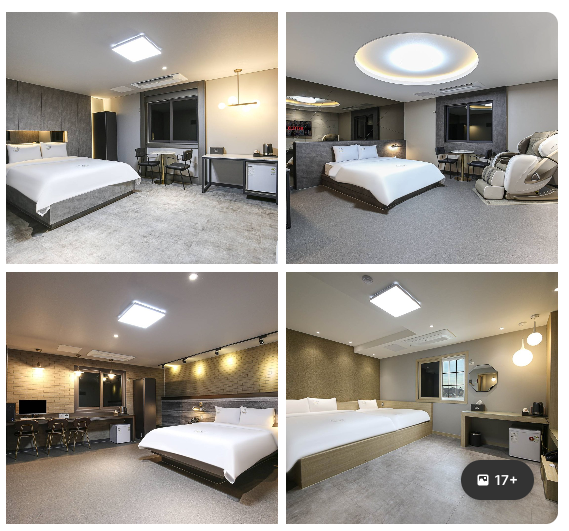
\includegraphics[width=\linewidth]{fig/5_방.png}
    \caption{방 사진}
    \label{fig:1}
  \end{subfigure}
  \hfill
  % 두 번째 그림
  \begin{subfigure}{0.3\textwidth}
    \centering
    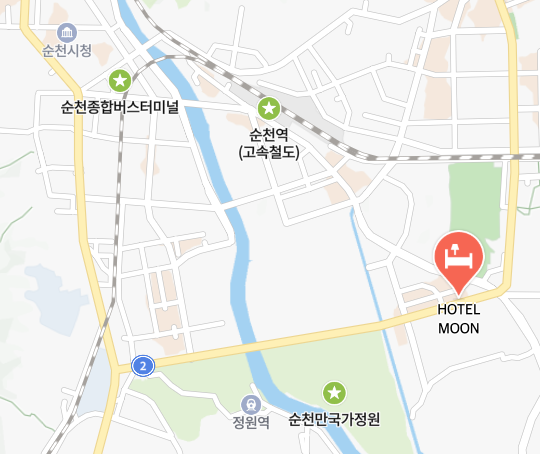
\includegraphics[width=\linewidth]{fig/5_위치.png}
    \caption{위치}
    \label{fig:2}
  \end{subfigure}
  \hfill
  % 세 번째 그림
  \begin{subfigure}{0.3\textwidth}
    \centering
    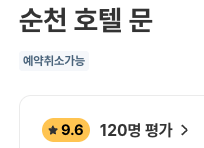
\includegraphics[width=\linewidth]{fig/5_후기.png}
    \caption{여기어때 후기}
    \label{fig:3}
  \end{subfigure}
  \label{fig:three}
\end{figure}
\begin{center}
\textbf{할인 적용 가격 : 60000}
\end{center}
\url{https://www.yeogi.com/domestic-accommodations/68433?checkIn=2025-08-02&checkOut=2025-08-03&personal=2}
\newpage
\section{Conclusion}
일단 내가 찜해둔것들 위주로 정리를 해두었는데, 3만원대로 가는거가 괜찮아 보이는것 같다. 
그리고 10만원대 (할인적용 6만원대) 숙소는 찾아보면 많다. 그니까 일단 이거 보고 3만원대로 갈지, 아니면 아싸리 6만원대로 갈지를 정해보고, 
6만원으로 갈거라면, 나무늘보 라던지 또 괜찮은것들도 많아 보인다. 

3만원대에서는 테라칸이나 써드호텔이 확실히 좋아보이고, 5만원대에서는 YAJA가 좀더 좋아보인다. 

\end{document}
